%! TeX program=latexmk
%! TeX options=-xelatex -synctex=1 -interaction=nonstopmode -file-line-error "%DOC%"
\documentclass[a4paper, nosysfonts]{hpcchina}
\usepackage{booktabs}
\usepackage{graphicx}
\usepackage{amsmath,amsthm}
\usepackage{amssymb,amsfonts}
\usepackage{makecell}
\usepackage{float}
\usepackage{array}
\usepackage{tabularx}
%以下宏包为测试用途
\usepackage{blindtext}
\usepackage{zhlipsum}
\usepackage{tikz}
\usepackage{metalogo}
%标题
\title{精仿HPC China \XeLaTeX 模板}
%作者
\author{段晓辉\textsuperscript{1,2}}
%单位
\affiliation{
  \textsuperscript{1} 清华大学,北京 100084
  
  \textsuperscript{2} 国家超级计算无锡中心,无锡 214072
}
%邮箱,使用\mailurl{地址}可以生成可点击的链接
\email{\mailurl{sunrise_duan@126.com}}
%中文摘要
\cabstract{
  \zhlipsum[1]
}
%中文关键词
\keyword{
  Latex模板;高性能计算
}
%英文标题
\etitle{DeepFake of HPC China Template in \XeLaTeX}
%英文作者
\eauthor{Xiaohui Duan\textsuperscript{1,2}}
%英文单位
\eaffiliation{
  \textsuperscript{1} (Tsinghua University, Beijing 100084)

  \textsuperscript{2} (National Supercomputing Center in Wuxi, Wuxi 214072)
}
%英文摘要
\eabstract{
  \blindtext[1]
}
%英文关键词
\ekeyword{
  Latex Template; High Performance Computing
}
%基金号
\grants{目前无人捐助此项目}
%DOI号
\doi{missing DOI}
%分类号
\clcls{TP391}
%卷(期):起止页,年
\issue{卷(期):起止页,年}
%收稿日期
\dateaccept{yyyy-mm-dd}
%修回日期
\daterevise{yyyy-mm-dd}
\begin{document}
    \maketitle
    
    \section{绪论}
    近年来,深度学习技术在计算机视觉、自然语言处理、医疗诊断等领域证明了其不可替代的价值,成为推动人工智能发展的中重要驱动力[1]。随着深度学习模型的不断发展和计算复杂度的持续增长,其训练和推理过程对底层计算硬件提出了更高要求。传统处理器(CPU)强调面向广泛任务的普适性,并行计算能力有限,难以满足现代深度学习算法的对计算能力和存储性能的巨大需求。这时将传统通用计算中低效的矩阵运算转化为高度并行的操作显得尤为重要,图形处理器(GPU)、张量处理单元(TPU)、现场可编程门阵列(FPGA)、专用集成电路(ASIC)等异构芯片纷纷涌现并不断迭代升级[2][3]


    国产智能芯片在近几年发展蓬勃,通过定制化的架构设计增强数据吞吐量和计算并行度,加速机器学习中的关键运算环节,大大提升深度学习模型的训练效率。然而在实际应用中,国产芯片很难发挥作用,其软件生态仍处于发展初期,缺乏成熟、高效的深度学习编译工具链,导致算子性能优化难度大。


    早期对深度学习模型的部署时,硬件厂商通常依赖人工针对硬件架构特点开发深度优化的算子库,如英特尔CPU的oneDNN[4]、英伟达GPU的cuDNN[5]等,此类手工调优方法虽然可以获得较高的性能,但存在开发周期长、维护成本高、移植能力差等显著缺点。因此,针对国产智能芯片架构特性设计一种具备自动调优能力、支持动态参数算子优化的代码生成器,不仅可突破传统手工调优的开发瓶颈,提升算子性能适配效率,更有助于补齐编译工具链短板,推动构建具有自主可控能力的国产深度学习软件生态,对促进人工智能技术的国产化应用具有重要现实意义与工程价值。

  \begin{figure}[!htbp]
  \centering
  \begin{tikzpicture}
    \node[draw] {\includegraphics[width=0.8\linewidth]{shenduxuexi.png}};
  \end{tikzpicture}
  \caption{深度学习编译器结构
    \ecaption{The Architecture of Deep Learning Compilers}
  }
\end{figure}


    本文的具体工作如下:

(1)选取一组具有代表性的元形状(meta shape)作为微内核(micro kernel),并为每个微内核分别训练对应的成本模型;

(2)利用成本模型的预测结果,从每个微内核中选取性能最优的Top-k参数设置,并求取这些参数配置的并集;

(3)将该参数并集作为通用参数搜索空间并应用到所有的测试形状上进行实际运行,最终选出性能最优的参数设置。
本章剩余内容安排如下:第二章为相关背景阐述,
    \section{背景}
    
    \subsection{人工智能芯片研究现状}
    人工智能技术致力于构能够模拟人类智能行为的计算系统,通过原始数据获取知识以处理通用问题或特定任务,推动人类社会向更高效、更智能的方向演进。最初的人工智能载体为在各个领域通用的CPU处理器,但随着性能要求的不断提升,CPU的算力几乎停滞不前,以CPU为核心的传统芯片已经难以满足深度学习高复杂任务的计算需求:例如,2016年Google的ALphaGo[7]与李世石围棋对弈时使用1202个CPU和176个GPU,每盘棋仅电力就需消耗数千美元。因此满足高性能、低功耗要求的承载人工智能核心技术的硬件基础——人工智能芯片应运而生。


    当前适合于深度学习任务的人工智能芯片可分为四大类型:通用图形处理器(GPU)、专用集成电路(ASIC)、半定制化硬件可编程门阵列(FPGA)以及类脑神经元结构芯片,其主要架构特点如下表2.1所示: 
\vspace{-1.8em}
    \begin{table}[H] 
  \centering
  \caption{不同人工智能芯片架构特点(Performance comparison of different AI chip architectures)}
  \begin{tabular}{lcccc}
    \toprule
    芯片类别 & GPU & FPGA & ASIC & 类脑芯片 \\
    \midrule
    特点 & \makecell{并行计算强\\能耗较高} 
        & \makecell{半定制化\\灵活性高} 
        & \makecell{全定制化\\性能高} 
        & \makecell{仿生神经结构\\低功耗} \\
    代表厂商 & \makecell{通用性强\\NVIDIA} 
            & \makecell{能效比中等\\Intel} 
            & \makecell{研发成本高\\寒武纪} 
            & \makecell{早期发展阶段\\IBM} \\
    \bottomrule
  \end{tabular}
\end{table}



    2014年陈云霁等人提出的DianNao[8]处理器作为首个深度学习专用处理器架构,将计算与存储进行了协同优化,其核心运算部件是由运算矩阵组成的三级流水线NFU(Neural Functional Unit)以实现高效的张量处理,存储方面创新性地采用分体式缓存架构,将片上存储分为神经元输入缓存(NBin)、神经元输出缓存(NBout)和突触缓存(SB)三部分独立管理,相比传统通用处理器CPU获得3个量级的能效提升,其架构如图2.1所示。2016年,谷歌公司正式发布其自主研发的神经网络专用加速器——张量处理单元TPU[10],其核心理念是通过引入大规模脉动阵列(Systolic Array)与大容量片上存储资源以实现对卷积类运算的高效加速,在脉动阵列满载时可达到极限计算性能,相较于Haswell CPU与NVIDIA K80 GPU,初代TPU在推理任务中展现出15至30倍的性能提升。2017年,英伟达推出Volta[11]架构,首次在GPU中引入了专为矩阵运算优化的计算单元Tensor Core,使神经网络的训练与推理性能比上一代的Pascal架构高3倍,增强了GPU的计算性能与程序性。目前TPU与Tensor Core均已迭代至多个版本,性能获得持续提升。其它国外互联网巨头如微软、亚马逊等也纷纷展开芯片业务。
    \begin{figure}[!htbp]
  \centering
  \begin{tikzpicture}
    \node[draw] {\includegraphics[width=0.8\linewidth]{diannao.png}};
  \end{tikzpicture}
  \caption{DianNao架构
    \ecaption{DianNao Architecture}
  }
\end{figure}
    \subsection{深度学习编译器与自动调优研究现状}
目前,深度学习编译器已经成为了深度学习领域的研究热点之一,其通用架构主要包括编译器前端和编译器后端两部分,如图2.2所示。前端部分基于高级中间表示(IR),主要处理与目标硬件无关的代码转换和优化,后端部分则基于低级IR,负责特定硬件的性能调优和代码生成[15],IR作为程序的抽象描述,为优化过程提供了关键支持。当下较为流行的深度学习编译器有TVM、XL、nGraph、TC、MLI和Triton等,接下来对其进行简要介绍。

TVM[16]是陈天奇等人提出的开源深度学习编译器平台,采用模块化设计,借鉴Halide的优化思想,将算法与调度解耦,并提供丰富的调度原语,使开发者可专注于模型设计。TVM使用Relay作为高级IR,Halide IR作为低级表示,支持量化类型与及动态形状处理。其后端具备针对不同硬件架构的代码生成与优化能力,包括循环变换、内存管理、特定指令映射等,并可集成cuDNN等高性能库。

XLA(Accelerated Linear Algebra)[17]是谷歌面向TensorFlow等框架开发的专用图编译器,旨在提升线性代数运算的执行效率。其核心机制是将神经网络的计算图映射为HLO中间表示,并围绕该IR执行包括常量折叠、表达式优化、算子融合、内存布局调整等优化策略。在后端阶段,XLA可调用cuDNN、MKL等高性能库实现算子的进一步加速,支持动态形状并通过JIT编译实现更高吞吐,或使用AOT编译以满足低延迟部署需求。nGraph[18]是英特尔开发的开源C++库,核心设计理念是将神经网络的计算图转化为静态的数据流图,通过图级优化与算子融合提高计算效率。nGraph使用高度抽象的IR构建优化与调度流程,并支持自动内存管理、常量传播、向量化等多种编译优化策略。在后端方面,nGraph可部署至英特尔的CPU、Nervana NNP等自家架构及OpenVINO工具链,更注重性能工程与对英特尔生态的深度整合,异构设备的支持有限。

TC(Tensor Comprehensions)[19]是Facebook推出的自动算子生成与优化框架。用户可通过简洁语法自定义张量计算公式,系统自动生成对应的CUDA或 LLVM IR,并结合基于polyhedral模型的调度策略优化执行流程。TC支持自动差分计算,可广泛应用于训练阶段,通过搜索方法生成高性能内核。其内部使用PPCG工具链进行polyhedral分析,优化循环结构和内存访问。然而,由于其对数学建模能力要求较高,开发门槛较大,加之项目长期未维护,实用性与生态活跃度有所下降。

MLIR(Multi-Level Intermediate Representation)[20]由Google提出,旨在为异构计算构建统一的中间表示基础。它支持多层次IR表达,可覆盖从高层框架到底层硬件指令的编译需求。通过采用方言机制,MLIR容许不同编译需求共存,使得如TensorFlow、XLA、Linalg、Affine等组件能在共享框架下交互。其设计鼓励开发者自定义优化策略,同时可实现跨编译阶段的内存管理、循环优化、张量转换等功能。MLIR强调模块复用、IR可组合性与扩展性,支持针对加速器、嵌入式平台的高效调度生成。

Triton[21]是OpenAI开源的高性能张量程序编译器,采用以tile为中心的中间表示和优化策略,支持通过Python风格的DSL编写自定义GPU内核。其编译流程涵盖Triton-C前端、基于LLVM的Triton-IR中间表示以及Triton-JIT后端,具备层次化tiling、内存访问合并、共享内存优化、自动预取和自动调优等能力,能够在无需深入CUDA编程经验的前提下实现近似cuDNN水平的执行效率。与传统深度学习编译器相比,Triton在复杂算子上表现出更强的灵活性和性能潜力,同时,其优化模型与调优机制具备较强的可迁移性,有望在寒武纪MLU370上实现高效的算子自动生成与部署,为国产智能芯片上的编译优化提供较为可行的技术路径。
    \subsection{寒武纪及国产芯片概况}
    在核心技术自主可控、地缘政治博弈等多重因素的驱动下,我国众多科技企业抓住开拓国内市场的机遇,争相布局国产智能芯片领域以实现关键算力资源的自主可控。

    寒武纪科技围绕Cambricon-1M架构开发了MLU(Machine Learning Unit)系列智能计算卡,并开发了BANGC语言作为框架的主要开发语言,同时提供兼容PyTorch[12]、TensorFlow[13]等主流深度学习框架的训练与推理软件栈,支持跨平台模型迁移。具体而言,开发者既可利用原生框架接口实现端到端模型训练,亦可通过标准化模型转换工具将异构计算设备训练的模型经结构重优化和量化压缩后部署至MLU硬件平台。其中思元370采用智能芯片架构MLUarch03,最大算力高达256TOPS(INT8),同时集成专有推理优化引擎MagicMind,采用基于计算图的中间表示(IR)进行算子融合、内存布局优化等编译期优化,显著提升模型在MLU架构上的推理效率和能效。

    华为推出晟腾人工智能处理器,称为NPU(Neural-network Processing Unit),系列产品包括搭载了晟腾910与晟腾310两款芯片的多种终端。其中,晟腾910主要面向云端场景,计算密度达到同期NVIDIA Tesla V100 GPU的两倍,与之配套的晟腾310专为边缘计算及移动终端设备优化。在架构设计方面,为适应深度神经网络的高密度矩阵运算需求,晟腾人工智能芯片采用“达芬奇架构”,通过3D Cube的设计在提升算力的同时优化能效比,对多维计算模式和多种类混合精度计算的支持使其在增加计算的灵活性的同时也强力支撑了数据的高精度要求。

    天数智芯通过“智铠+天垓”构建了推理与训练协同发展的国产智能芯片体系,其中,智铠系列采用通用GPU架构及通用指令集,针对推理应用,指令效率高、算力密度大,优化了计算与存储的平衡。天垓系列产品采用通用GPU架构,兼容国际主流GPU通用计算模型,支持国内外主流人工智能生态和深度学习框架及原生算子,具备应用覆盖广、性能可预期、开发易迁移以及全栈可定制等特点。


    \subsubsection{三级标题}
    \zhlipsum[10]
    \section{图表}
    \zhlipsum[2]
    \zhlipsum[1]
    %插图还是用figure
    \begin{figure}[!htbp]
      \centering
      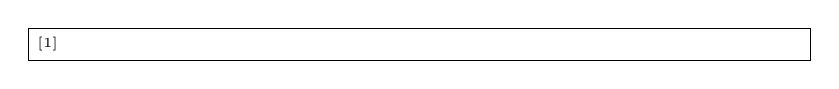
\begin{tikzpicture}
        \node[draw] {\parbox{.8\linewidth}{\tiny\zhlipsum[1]}};
      \end{tikzpicture}
      \caption{一张tikzpicture
        %英文caption用ecaption嵌在caption里面
        \ecaption{A tikzpicture}
      }
    \end{figure}
    \zhlipsum[1]
    %表应该用table也没啥问题
    \begin{table}[!htbp]
      \centering
      \caption{生成奇怪文字所用的库
        \ecaption{Library for generating strange text}
      }
      \begin{tabular}{|c|c|c|}\hline
        语言 & 库 & 命令\\\hline
        中文 & zhlipsum & \verb|\zhlipsum[段落数]|\\\hline
        English & blindtext & \verb|\blindtext[段落数]|\\\hline
      \end{tabular}
    \end{table}
    %表应该用table也没啥问题
    \begin{table}[!htbp]
      \centering
      \caption{ecaption的支持情况
        \ecaption{Supported ecaptions}
      }
      \begin{tabular}{|c|c|c|}\hline
        类型 & 中文 & 英文\\\hline
        figure & 图 x& Fig. x\\\hline
        table & 表 x& Table x\\\hline
        其他 & & 定义方式类似:\\
         &  & \verb|\ecaptionname{figure}{Fig.}|\\\hline
      \end{tabular}
    \end{table}
    \zhlipsum[1-5]
    以一篇古老的分子动力学文章作为参考\cite{jones1924on}
    %参考文献
    \bibliography{ref.bib}
    %作者简介{照片}{文字},可以用includegraphics代替tikzpicture,照片自动缩放
    \authorbio{
      \begin{tikzpicture}\node[minimum width=0.6in, minimum height=0.8in, draw]{照片};\end{tikzpicture}
    }{\textbf{段晓辉} 国家超级计算无锡中心,高级研发工程师,擅长\LaTeX 编程。}


    \authorbio{
      \includegraphics{123.png}
    }{
      This work is licensed under a \href{http://creativecommons.org/licenses/by-nc/4.0/}{Creative Commons Attribution-NonCommercial 4.0 International License}.
    }
\end{document}


